\documentclass[xetex,mathserif,serif,aspectratio=169]{beamer}

\usepackage{xltxtra}
\usepackage{color}
\usepackage{url}
\usepackage{listings}
\usepackage{fontspec}
\usepackage{geometry}
\usepackage{lastpage}
\usepackage{fancyhdr}
\usepackage{amsmath}
\usepackage{amsthm}
\usepackage{amssymb}
\usepackage{blkarray}
\usepackage{multicol}
\usepackage{relsize}
\usepackage{listings}
\usepackage{xunicode}
\usepackage{xltxtra}
\usepackage{color}
\usepackage{url}
\usefonttheme[onlymath]{serif}

\definecolor{solarized@base03}{HTML}{002B36}
\definecolor{solarized@base02}{HTML}{073642}
\definecolor{solarized@base01}{HTML}{586e75}
\definecolor{solarized@base00}{HTML}{657b83}
\definecolor{solarized@base0}{HTML}{839496}
\definecolor{solarized@base1}{HTML}{93a1a1}
\definecolor{solarized@base2}{HTML}{EEE8D5}
\definecolor{solarized@base3}{HTML}{FDF6E3}
\definecolor{solarized@yellow}{HTML}{B58900}
\definecolor{solarized@orange}{HTML}{CB4B16}
\definecolor{solarized@red}{HTML}{DC322F}
\definecolor{solarized@magenta}{HTML}{D33682}
\definecolor{solarized@violet}{HTML}{6C71C4}
\definecolor{solarized@blue}{HTML}{268BD2}
\definecolor{solarized@cyan}{HTML}{2AA198}
\definecolor{solarized@green}{HTML}{859900}
\definecolor{yaleblue}{HTML}{0E4C92}

\newcommand{\yellow}[1]{\textcolor{solarized@yellow}{#1}}
\newcommand{\orange}[1]{\textcolor{solarized@orange}{#1}}
\newcommand{\red}[1]{\textcolor{solarized@red}{#1}}
\newcommand{\magenta}[1]{\textcolor{solarized@magenta}{#1}}
\newcommand{\violet}[1]{\textcolor{solarized@violet}{#1}}
\newcommand{\blue}[1]{\textcolor{solarized@blue}{#1}}
\newcommand{\cyan}[1]{\textcolor{solarized@cyan}{#1}}
\newcommand{\green}[1]{\textcolor{solarized@green}{#1}}
\newcommand{\yblue}[1]{\textcolor{yaleblue}{#1}}
\newcommand{\base}[1]{\textcolor{solarized@base01}{#1}}


\defaultfontfeatures{Mapping=tex-text}
\hypersetup{pdfstartview={FitH}}

\newcommand{\old}[1]{\fontspec[Alternate=1,Ligatures={Common}]{Hoefler Text}\fontsize{18pt}{30pt}\selectfont #1}%
\newcommand{\oldA}[1]{\fontspec[Alternate=1,Ligatures={Common, Rare}]{Hoefler Text}\fontsize{12pt}{15pt}\selectfont #1}%
\newcommand{\oldB}[1]{\fontspec[Ligatures={Common}]{Didot}\fontsize{12pt}{15pt}\color{solarized@base02}\selectfont #1}%
\newcommand{\tfont}[1]{\fontspec[Alternate=1,Ligatures={Common}]{Hoefler Text}\fontsize{12pt}{20pt}\selectfont #1}%
\newcommand{\dfont}[1]{\fontspec[Ligatures={Common}]{Didot}\fontsize{12pt}{12pt}\selectfont #1}%

\setbeamerfont{title}{family=\old}
\setbeamerfont{author}{family=\tfont}%
\setbeamerfont{frametitle}{family=\oldA}
\setbeamerfont{date}{family=\dfont}

\setbeamertemplate{navigation symbols}{}
\setbeamertemplate{footline}[text line]{%
  \parbox{0.99\linewidth}{
    \normalsize\vspace*{-24pt}\hfill{\color{solarized@base00}\insertframenumber/\inserttotalframenumber}
  }
}


\setlength{\parindent}{0pt}
\setlength{\parskip}{12pt}

\setbeamercolor{structure}{bg=solarized@base3, fg=solarized@base02}
\setbeamercolor{titlelike}{fg=solarized@cyan}
\setbeamercolor{title}{fg=solarized@blue}
\setbeamercolor{subtitle}{fg=solarized@magenta}
\setbeamercolor{alerted text}{fg=orange}
\setbeamercolor{itemize}{fg=solarized@base02}
\setbeamercolor{background canvas}{bg=solarized@base3}
\setbeamercolor{enumerate subitem}{fg=solarized@base02}

\newcommand{\minimize}{\mathop{\mathrm{minimize}}}
\newcommand{\argmin}{\mathop{\mathrm{arg\,min}}}
\newcommand{\argmax}{\mathop{\mathrm{arg\,max}}}
\newcommand{\st}{\mathop{\mathrm{subject\,\,to}}}


\usepackage[]{algorithm2e}
\usepackage{../kbordermatrix}

\begin{document}

%%%%%%%%%%%%%%%%%%%%%%%%%%%%%%%%%%%%%%%%%%%%%%%%%%%
\begin{frame}[fragile] \frametitle{} \oldB \small

\vfill

{\fontsize{0.7cm}{0cm}\selectfont Lecture 06 \\\vspace{0.2cm} Decision Trees I}\\\vspace{0.5cm}
08 February 2016

\vspace{2cm}

\begin{minipage}{0.6\textwidth}
Taylor B. Arnold \\
Yale Statistics \\
STAT 365/665
\end{minipage}
\hfill
\begin{minipage}{0.3\textwidth}\raggedleft

\includegraphics[scale=0.3]{../yale-logo.png}
\end{minipage}%

\end{frame}

%%%%%%%%%%%%%%%%%%%%%%%%%%%%%%%%%%%%%%%%%%%%%%%%%%%
\begin{frame}[fragile] \frametitle{} \oldB \small

\begin{itemize}
\item Problem Set \#2 Posted -- Due February 19th
\item Piazza site \url{https://piazza.com/}
\end{itemize}

\end{frame}

%%%%%%%%%%%%%%%%%%%%%%%%%%%%%%%%%%%%%%%%%%%%%%%%%%%
\begin{frame}[fragile] \frametitle{} \oldB \small

Last time we starting fitting additive models to the variables
in the California pricing data.

As I alluded to, it actually makes more sense to allow an
interaction between latitude and longitude. This is easy
to include in \texttt{mgcv}:
\begin{lstlisting}[language=R, basicstyle=\ttfamily]
> ca <- read.csv("ca.csv", as.is=TRUE)
> library(mgcv)
> ca.gam2 <- gam(log(median_house_value)
+   ~ s(median_household_income) + s(mean_household_income)
+   + s(population) + s(total_units) + s(vacant_units)
+   + s(owners) + s(median_rooms) + s(mean_household_size_owners)
+   + s(mean_household_size_renters)
+   + s(longitude,latitude), data=ca, subset=trainFlag)
\end{lstlisting}

\end{frame}

%%%%%%%%%%%%%%%%%%%%%%%%%%%%%%%%%%%%%%%%%%%%%%%%%%%
\begin{frame}[fragile] \frametitle{} \oldB \small

\begin{center}
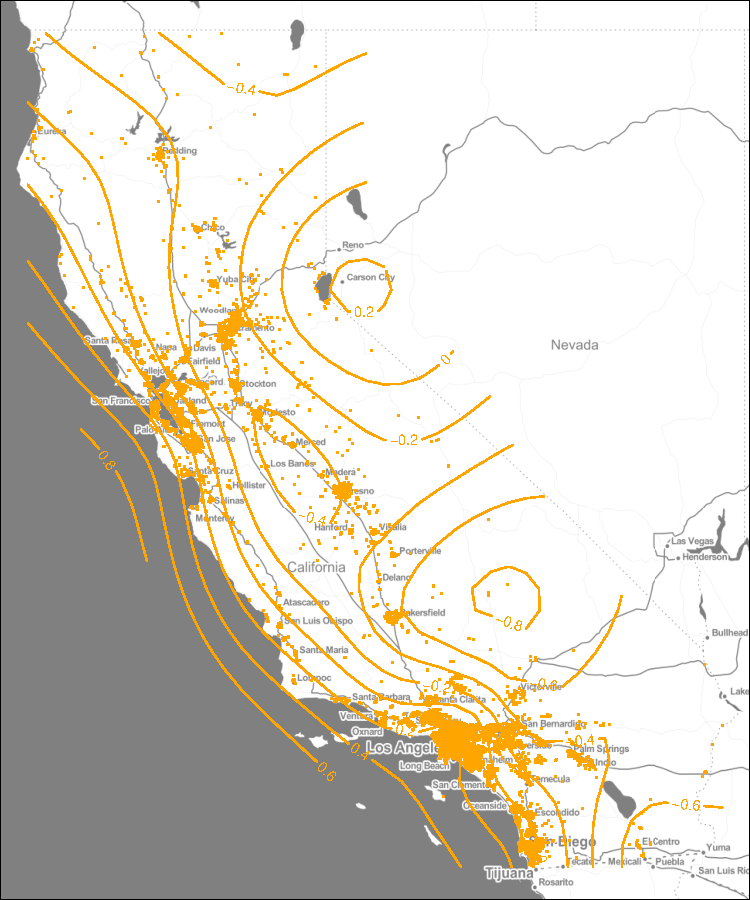
\includegraphics[height=\textheight]{img/fig03.pdf}
\end{center}

\end{frame}

%%%%%%%%%%%%%%%%%%%%%%%%%%%%%%%%%%%%%%%%%%%%%%%%%%%
\begin{frame}[fragile] \frametitle{} \oldB \small

How well does these methods do in terms of prediction? We can
predict using the \texttt{predict} function just as with linear
models:
\begin{lstlisting}[language=R, basicstyle=\ttfamily]
> y <- log(ca$median_house_value)
> ca.lm.pred <- predict(ca.lm, ca)
> ca.gam.pred <- predict(ca.gam, ca)
> ca.gam2.pred <- predict(ca.gam2, ca)
\end{lstlisting}
And then check the mean squared error on both the
training set and testing set:
\begin{lstlisting}[language=R, basicstyle=\ttfamily]
> tapply((ca.lm.pred - y)^2, trainFlag, mean)
FALSE  TRUE
0.096 0.101
> tapply((ca.gam.pred - y)^2, trainFlag, mean)
FALSE  TRUE
0.064 0.072
> tapply((ca.gam2.pred - y)^2, trainFlag, mean)
FALSE  TRUE
0.059 0.065
\end{lstlisting}

\end{frame}


%%%%%%%%%%%%%%%%%%%%%%%%%%%%%%%%%%%%%%%%%%%%%%%%%%%
\begin{frame}[fragile] \frametitle{} \oldB \small

In machine learning, you'll often hear the caveat that our conclusions
always depends on future values following \magenta{the same underlying model}.
I think we say that a lot, but forget to really think about it.
To illustrate, let's re-fit the model on the California data without
the latitude and longitude components. We can then see how well the
model trained on California data generalizes to Pennsylvania data.

\end{frame}

%%%%%%%%%%%%%%%%%%%%%%%%%%%%%%%%%%%%%%%%%%%%%%%%%%%
\begin{frame}[fragile] \frametitle{} \oldB \small

Here are the two linear models fit on the two different datasets.
\begin{lstlisting}[language=R, basicstyle=\ttfamily]
> ca.lm2 <- lm(log(median_house_value) ~ median_household_income
+   + mean_household_income + population + total_units +
+   + vacant_units + owners + median_rooms +
+   + mean_household_size_owners + mean_household_size_renters,
+   data = ca, subset=trainFlag)
>
> pa.lm3 <- lm(log(median_house_value) ~ median_household_income
+   + mean_household_income + population + total_units +
+   + vacant_units + owners + median_rooms +
+   + mean_household_size_owners + mean_household_size_renters,
+   data = pa, subset=trainFlagPa)
\end{lstlisting}

\end{frame}


%%%%%%%%%%%%%%%%%%%%%%%%%%%%%%%%%%%%%%%%%%%%%%%%%%%
\begin{frame}[fragile] \frametitle{} \oldB \small

And here are the two additive models fit on the two datasets:
\begin{lstlisting}[language=R, basicstyle=\ttfamily]
> ca.gam3 <- gam(log(median_house_value)
+   ~ s(median_household_income) + s(mean_household_income)
+   + s(population) + s(total_units) + s(vacant_units)
+   + s(owners) + s(median_rooms) + s(mean_household_size_owners)
+   + s(mean_household_size_renters), data=ca, subset=trainFlag)
>
> pa.gam4 <- gam(log(median_house_value)
+   ~ s(median_household_income) + s(mean_household_income)
+   + s(population) + s(total_units) + s(vacant_units)
+   + s(owners) + s(median_rooms) + s(mean_household_size_owners)
+   + s(mean_household_size_renters), data=pa, subset=trainFlagPa)
\end{lstlisting}

\end{frame}

%%%%%%%%%%%%%%%%%%%%%%%%%%%%%%%%%%%%%%%%%%%%%%%%%%%
\begin{frame}[fragile] \frametitle{} \oldB \small

Finding the predicted values from these models all on the PA data:
\begin{lstlisting}[language=R, basicstyle=\ttfamily]
> y.pa <- log(pa$median_house_value)
> pa.lm2.pred <- predict(ca.lm2, pa)
> pa.gam3.pred <- predict(ca.gam3, pa)
> pa.lm3.pred <- predict(pa.lm3, pa)
> pa.gam4.pred <- predict(pa.gam4, pa)
\end{lstlisting}

\end{frame}


%%%%%%%%%%%%%%%%%%%%%%%%%%%%%%%%%%%%%%%%%%%%%%%%%%%
\begin{frame}[fragile] \frametitle{} \oldB \small

We see that the California ones yield very poor MSE scores
for PA:
\begin{lstlisting}[language=R, basicstyle=\ttfamily]
> tapply((pa.lm2.pred - y.pa)^2,trainFlagPa,mean)
FALSE  TRUE
 0.58  0.55
> tapply((pa.gam3.pred - y.pa)^2,trainFlagPa,mean)
FALSE  TRUE
 0.47  0.44
\end{lstlisting}
Compared to those models trained on the PA data:
\begin{lstlisting}[language=R, basicstyle=\ttfamily]
> tapply((pa.lm3.pred - y.pa)^2,trainFlagPa,mean)
FALSE  TRUE
0.095 0.093
> tapply((pa.gam4.pred - y.pa)^2,trainFlagPa,mean)
FALSE  TRUE
0.070 0.063
\end{lstlisting}

\end{frame}

%%%%%%%%%%%%%%%%%%%%%%%%%%%%%%%%%%%%%%%%%%%%%%%%%%%
\begin{frame}[fragile] \frametitle{} \oldB \small

However, if we account for the overall means being different, we
see that the California models perform reasonably well on
the Pennsylvania data:
\begin{lstlisting}[language=R, basicstyle=\ttfamily]
> tapply((pa.lm2.pred - y.pa),trainFlagPa,var)
FALSE  TRUE
 0.14  0.13
> tapply((pa.gam3.pred - y.pa),trainFlagPa,var)
FALSE  TRUE
0.094 0.084
> tapply((pa.lm3.pred - y.pa),trainFlagPa,var)
FALSE  TRUE
0.095 0.093
> tapply((pa.gam4.pred - y.pa),trainFlagPa,var)
FALSE  TRUE
0.070 0.063
\end{lstlisting}

\end{frame}

%%%%%%%%%%%%%%%%%%%%%%%%%%%%%%%%%%%%%%%%%%%%%%%%%%%
\begin{frame}[fragile] \frametitle{} \oldB \small

\begin{flushright}
{\color{yaleblue}\sc\fontsize{1cm}{0cm}\selectfont Tree-Based Models}
\end{flushright}

\end{frame}

%%%%%%%%%%%%%%%%%%%%%%%%%%%%%%%%%%%%%%%%%%%%%%%%%%%
\begin{frame}[fragile] \frametitle{} \oldB \small

In order to deal with the combinatorial explosion of modeling every
interaction in higher-dimensional non-parametric regression and classification
models, we have seen that \blue{additive models} assume that there are
no interactions between the input variables.

\pause \blue{Tree-based models} instead allow interactions, but use the
data to greedily determine which interactions to include.

\end{frame}

%%%%%%%%%%%%%%%%%%%%%%%%%%%%%%%%%%%%%%%%%%%%%%%%%%%
\begin{frame}[fragile] \frametitle{} \oldB \small

I think it is easiest to understand tree models by first seeing an example
before backing into the formal definition of how these models are fit.

\begin{lstlisting}[language=R, basicstyle=\ttfamily]
> tf <- tree(log(median_house_value) ~ longitude + latitude, data = ca)
> plot(tf)
> text(tf, cex=0.75)
\end{lstlisting}

\end{frame}

%%%%%%%%%%%%%%%%%%%%%%%%%%%%%%%%%%%%%%%%%%%%%%%%%%%
\begin{frame}[fragile] \frametitle{} \oldB \small

\begin{center}
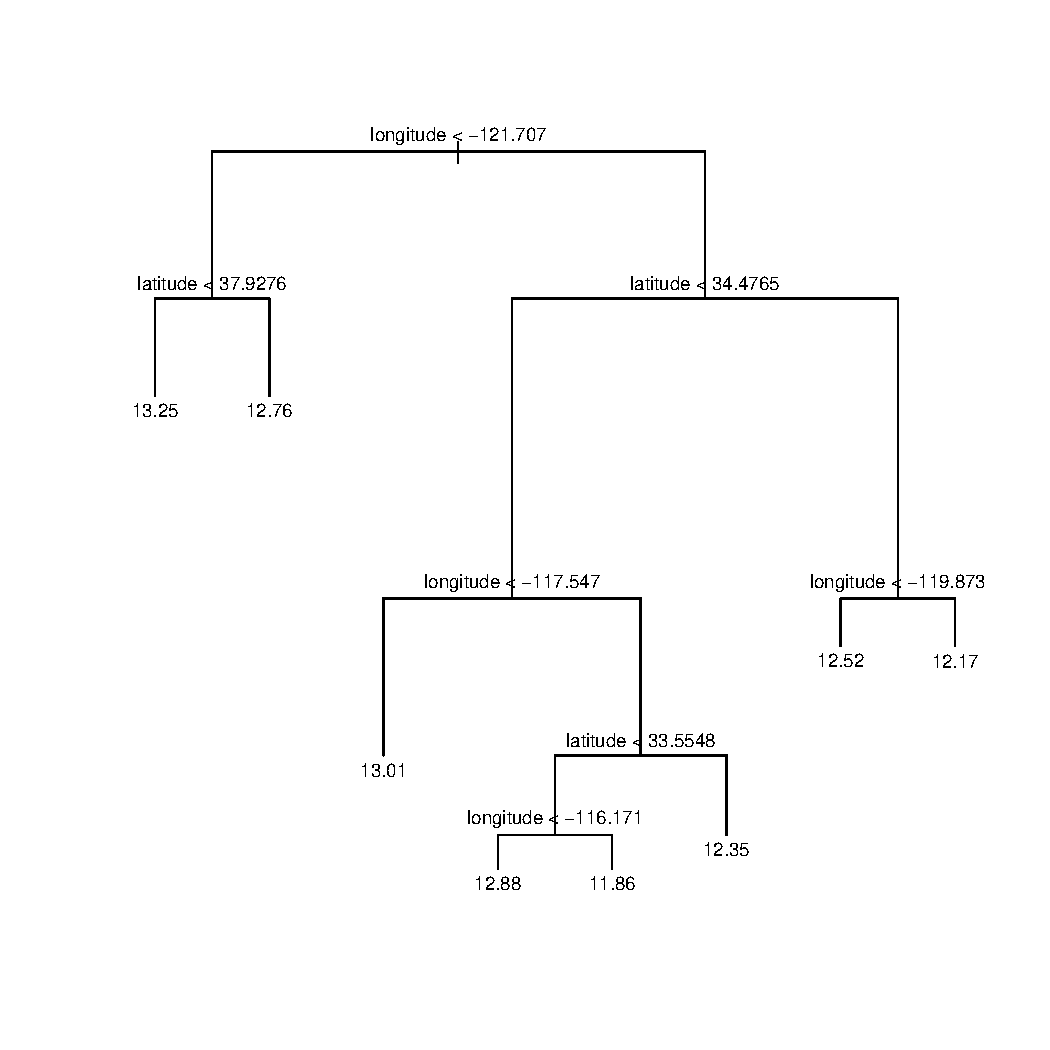
\includegraphics[height=\textheight]{img/simpleTree.pdf}
\end{center}

\end{frame}

%%%%%%%%%%%%%%%%%%%%%%%%%%%%%%%%%%%%%%%%%%%%%%%%%%%
\begin{frame}[fragile] \frametitle{} \oldB \small

\begin{center}
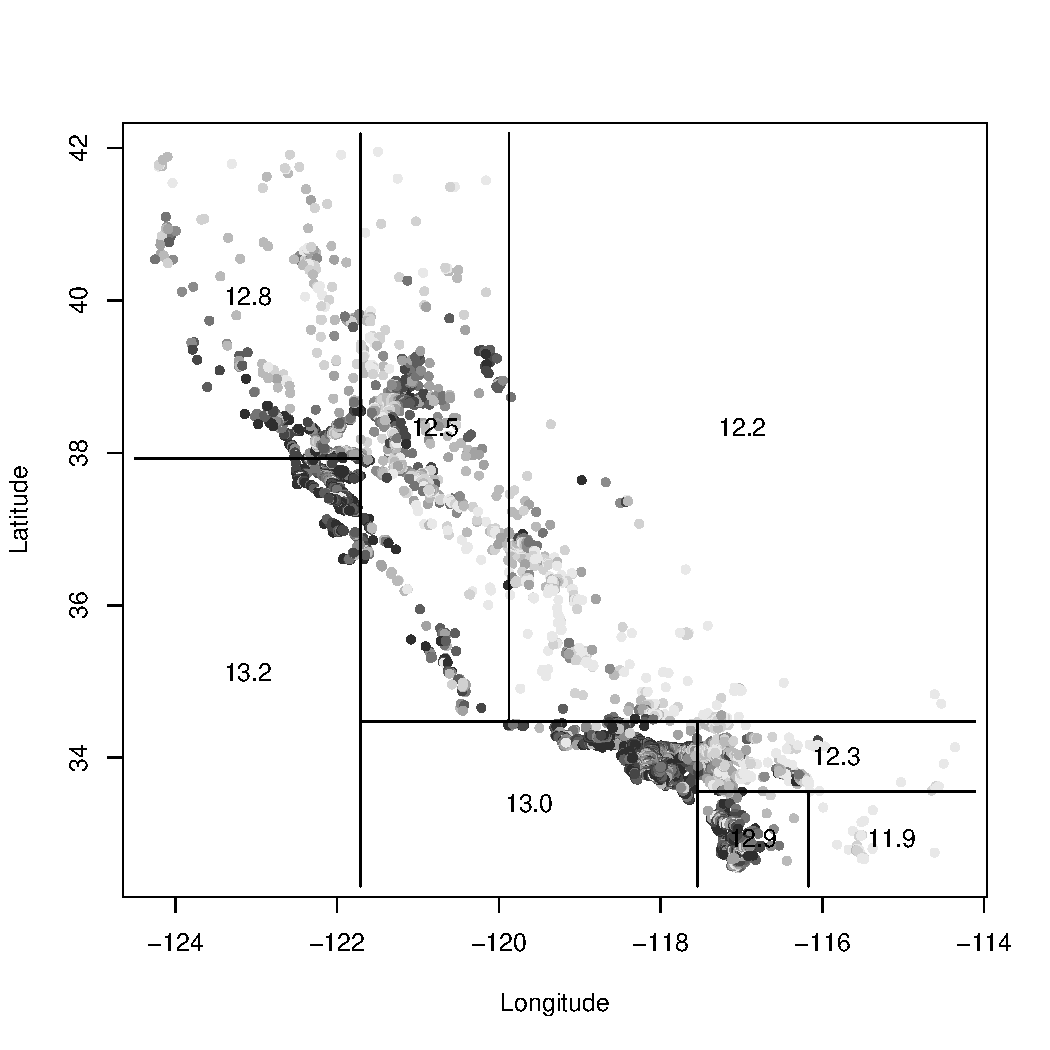
\includegraphics[height=\textheight]{img/simplePartTree.pdf}
\end{center}

\end{frame}

%%%%%%%%%%%%%%%%%%%%%%%%%%%%%%%%%%%%%%%%%%%%%%%%%%%
\begin{frame}[fragile] \frametitle{} \oldB \small

\textbf{\yblue{Regression trees}}

The fitting algorithm for learning such a tree is as follows:
\begin{enumerate}
\item Consider splitting on every possible unique value of every
single variable in the data. Pick the `best' split from amongst
all of these options.\pause
\item Partition the training data into two classes based on step $1$.\pause
\item Now, iteratively apply step $1$ separately to each partition of
the data.\pause
\item Continue splitting each subset until an appropriate
stopping criteria has been reached.\pause
\item Calculate the mean of all the training data in a terminal node
(i.e., `leaf') of the learned tree structure. Use this as the predicted
value for future inputs that fall within the same bucket.
\end{enumerate}

\end{frame}

%%%%%%%%%%%%%%%%%%%%%%%%%%%%%%%%%%%%%%%%%%%%%%%%%%%
\begin{frame}[fragile] \frametitle{} \oldB \small

\textbf{\yblue{Stopping criterion}}

There are many commonly used stopping criterion, often used
simultaneously (if any is satisfied stop splitting the partition):
\begin{enumerate}
\item minimum number of training samples in a node
\item maximum number of splits
\item minimum improvement in the best split
\item maximum depth of the tree
\end{enumerate}
In practice, particularly for larger datasets, the maximum number
of splits is the mostly commonly used.

\end{frame}

%%%%%%%%%%%%%%%%%%%%%%%%%%%%%%%%%%%%%%%%%%%%%%%%%%%
\begin{frame}[fragile] \frametitle{} \oldB \small

\textbf{\yblue{Measuring `best' splits}}

A simple way of measuring how good a partition of the dataset is
is to use the residual sum of squares from the predicted values that would
be implied by the partition. So for the partition $I$, we have:
\begin{align*}
\sum_{i \in I} (y_i - \Sigma_{i \in I}(y_i))^2 + \sum_{i \notin I} (y_i - \Sigma_{i \notin I}(y_i))^2
\end{align*}

\end{frame}

%%%%%%%%%%%%%%%%%%%%%%%%%%%%%%%%%%%%%%%%%%%%%%%%%%%
\begin{frame}[fragile] \frametitle{} \oldB \small

\textbf{\yblue{Measuring `best' splits, cont.}}

Notice that using the standard trick with variance calculations we
can simplify this. Setting $\Sigma_{i \in I}(y_i) = \bar{y}_{I}$,
$\Sigma_{i \notin I}(y_i) = \bar{y}_{I^c}$ and $n_I$ and $n_{I^c}$ as
the sample sizes of the partitions, we have:
\begin{align*}
\sum_{i \in I} (y_i - \bar{y}_{I})^2 + \sum_{i \notin I} (y_i - \bar{y}_{I^c})^2
&= \sum_{i \in I} \left(y_i^2 + \bar{y}_{I}^2 - 2y_i\bar{y}_{I}  \right) +
   \sum_{i \notin I} \left(y_i^2 + \bar{y}_{I^c}^2 - 2y_i\bar{y}_{I^c}  \right) \\
&= \sum_{i \in I} \left( y_i \right)^2 -  n_I \cdot \bar{y}_{I}^2 +
   \sum_{i \notin I} \left( y_i \right)^2 - n_{I^c} \cdot \bar{y}_{I^c}^2  \\
&=  \sum_{i} \left( y_i \right)^2 - n_I \cdot \bar{y}_{I}^2 - n_{I^c} \cdot \bar{y}_{I^c}^2
\end{align*}
\pause The first term does not change, so the goal is to actually minimize the
following:
\begin{align*}
\argmax_{\forall I} \frac{1}{n_I} \cdot \left( \sum_{i \in I} y_i \right)^2 +
\frac{1}{n_{I^c}} \cdot \left( \sum_{i \notin I} y_i \right)^2
\end{align*}

\end{frame}

%%%%%%%%%%%%%%%%%%%%%%%%%%%%%%%%%%%%%%%%%%%%%%%%%%%
\begin{frame}[fragile] \frametitle{} \oldB \small

\textbf{\yblue{Computational details}}

If we sort the responses $y_i$ such that their corresponding $x$ values are
increasing for a particular variable, we can write this even more compactly as:
\begin{align*}
\argmax_{j = 1, 2, \ldots n-1} \left\{ \frac{1}{j} \cdot \left( \sum_{i \leq j} y_i \right)^2 +
\frac{1}{n - j} \cdot \left( \sum_{i > j} y_i \right)^2 \right\}
\end{align*}
If we are clever, these can be calculated in only $\magenta{\mathcal{O}(n)}$
operations.

\pause If we have a maximum of $K$ splits, the total computational cost of
fitting a regression tree can be bounded by $\magenta{\mathcal{O}(np \cdot (\log(n) + K))}$,
but requires us to store $p$ copies of the $n$ response variables.

\end{frame}

%%%%%%%%%%%%%%%%%%%%%%%%%%%%%%%%%%%%%%%%%%%%%%%%%%%
\begin{frame}[fragile] \frametitle{} \oldB \small

\textbf{\yblue{Trees as Adaptive knn}}

Notice that the final predictions of a decision tree amount to simply
averaging all of responses for samples that are in a given bucket. In
this way, trees are like k-nearest neighbors, except that what defines
`near' is learned from the data rather than blindly using distances in
the x-space\ldots This helps to combat the curse of dimensionality but
may over-fit the training data.

Note that decision trees are \textbf{not} linear smoothers because the
weights are not independent functions of the x values.

\end{frame}

%%%%%%%%%%%%%%%%%%%%%%%%%%%%%%%%%%%%%%%%%%%%%%%%%%%
\begin{frame}[fragile] \frametitle{} \oldB \small

\textbf{\yblue{Classification trees}}

By coding a class label as $\pm 1$, and using the one-vs-many trick, we
can directly apply the regression tree algorithm to classification problems.
This actually works fine for two class problems, but is inefficient for
multi-class ones. It is better to instead use a measurement of the goodness
of a partition that directly includes all of the class labels. Choices
include mutual entropy and multinomial deviance.

\end{frame}

%%%%%%%%%%%%%%%%%%%%%%%%%%%%%%%%%%%%%%%%%%%%%%%%%%%
\begin{frame}[fragile] \frametitle{} \oldB \small

\textbf{\yblue{Categorical and ordinal prediction variables}}

If a predictor variable is an \blue{ordinal} variable, such as letter
grades or terms such as `low', `medium' and `high', these can be
mapped to numerical values in a natural way in tree based models.

Unordered categorical variables can be converted to factor levels as
in a linear regression, however there is another option: when considering
the split points of the categorical variable simply choose between all
possible permutations of the categories. This is feasible for up to
several dozen variables, depending on the amount of data and how long
you are willing to wait on the results.

\end{frame}

%%%%%%%%%%%%%%%%%%%%%%%%%%%%%%%%%%%%%%%%%%%%%%%%%%%
\begin{frame}[fragile] \frametitle{} \oldB \small

\textbf{\yblue{Why trees?}}

\begin{itemize}
\item able to interpret the important variables in a model
\item handles missing values well in both training and testing data
\item reasonably fast to train
\item does not depend on the scale of the predictor variables
\item can handle multiclass problems directly
\item works natively with categorical variables
\item easily modified to be robust to outliers (just replace MSE with MAD
for evaluating splits; means with medians for predictions in terminal nodes)
\item very fast to classify new points
\item robust to tuning parameters (the stopping criteria), \textit{for a given set of data}
\end{itemize}

\end{frame}

%%%%%%%%%%%%%%%%%%%%%%%%%%%%%%%%%%%%%%%%%%%%%%%%%%%
\begin{frame}[fragile] \frametitle{} \oldB \small

\textbf{\yblue{Stability}}

Regression and classification trees are robust to the stopping criterion,
but very sensitive to the input data used from training. Removing some
small fraction, say 10\%, of the training data can often lead to an
extremely different set of predictions.

Fortunately, we can use this instability to our advantage!

\end{frame}

%%%%%%%%%%%%%%%%%%%%%%%%%%%%%%%%%%%%%%%%%%%%%%%%%%%
\begin{frame}[fragile] \frametitle{} \oldB \small

\textbf{\yblue{Random forests}}

Random forests fit many decision trees to the same training data.
Each decision tree is fit using the aforementioned procedure except
that:
\begin{itemize}
\item the training set for a given tree is sampled from the original
data, with or without replacement
\item at each training split, only a randomly chosen subset (of size $m$)
of the variable are considered for splitting the data
\end{itemize}
In order to predict new values from this ensemble of trees, we take the
predictions from each model and average them together (for classification,
the class labels can also be used as `votes').

\end{frame}

%%%%%%%%%%%%%%%%%%%%%%%%%%%%%%%%%%%%%%%%%%%%%%%%%%%
\begin{frame}[fragile] \frametitle{} \oldB \small

\textbf{\yblue{Random forest tuning parameters}}

The main tuning parameters for random forests are the total number of
trees $T$, the maximum depth of the trees $K$ and the number of variables
$m$ randomly chosen to be available at each split.

Conveniently, $T$ and $K$ typically just need to be large enough and
so are relatively easy to set in practice. Values of $m$ typically range
from $\sqrt{m}$ up to $m/3$. This parameter can have a large effect on
the model, but is also generally easy to find a reasonable value and
not extremely sensitive in most cases.

\end{frame}

%%%%%%%%%%%%%%%%%%%%%%%%%%%%%%%%%%%%%%%%%%%%%%%%%%%
\begin{frame}[fragile] \frametitle{} \oldB \small

\textbf{\yblue{Random forest, computational details}}

Random forests have three very convenient computational benefits. First
of all, each tree is learned independently and so can be fit in parallel.
Over a cluster this requires a local copy of the data, but on a single
machine the data can be shared across workers as the raw data is never
modified.

Secondly, the sorting scheme we described earlier, where the sample
responses are sorted based on each variable, can be (carefully) used
as-is for each tree. That is, we only need to sort the data once and
can use this sorted set for each tree. We just simply apply weights
to this set according the sampling scheme used on each tree.

Finally, the fact that we only need to consider $m$ variables at each
split reduces the cost of fitting a given tree.

\end{frame}

%%%%%%%%%%%%%%%%%%%%%%%%%%%%%%%%%%%%%%%%%%%%%%%%%%%
\begin{frame}[fragile] \frametitle{} \oldB \small

\textbf{\yblue{Random forest, computational details, cont.}}

In total, a random forest can be fit in
\begin{align*}
\magenta{\mathcal{O}(np\log(p) + (KT) \cdot (mn))}
\end{align*}
operations when running serially. Using $C$ parallel cores, this can reduced
to only:
\begin{align*}
\magenta{\mathcal{O}(np\log(p) + (KT/C) \cdot (mn))}
\end{align*}

\end{frame}

%%%%%%%%%%%%%%%%%%%%%%%%%%%%%%%%%%%%%%%%%%%%%%%%%%%
\begin{frame}[fragile] \frametitle{} \oldB \small

\textbf{\yblue{Random forest, computational details, cont.}}

If the data is too large to fit into memory, one can set the
sub-sampling rate small enough to allow each tree to load its data into memory
(though this requires re-sorting each time). Alternatively, each node in
a cluster can locally run a random forest only on its individual chunk of data;
this often produces reasonable results.

There are also some completely different approaches which either involve
very low latency message passing at each node, or discretizing the input
variables and representing the problem at each node as a two-way table
(see MLLib for an example of the latter).

\end{frame}

%%%%%%%%%%%%%%%%%%%%%%%%%%%%%%%%%%%%%%%%%%%%%%%%%%%
\begin{frame}[fragile] \frametitle{} \oldB \small

\textbf{\yblue{Out-of-bag error}}

Notice that for any given observation $i$, there should be a
set of the trees in a random forest such that $i$ was not
randomly chosen to train them. Because $i$ was not used to
train these trees, if we look at only the predictions from
this set and compare it to $y_i$, this is an unbiased view
of how good the tree is fitting the data.

Using these predicted values for each $i$, we can efficiently
calculate a variant of cross-validation. This is called the
\magenta{out-of-bag error}.

\end{frame}

%%%%%%%%%%%%%%%%%%%%%%%%%%%%%%%%%%%%%%%%%%%%%%%%%%%
\begin{frame}[fragile] \frametitle{} \oldB \small

\textbf{\yblue{Variable importance}}

We can associated each node with a score indicating how much
that node decreased the overall mean squared error of the
training data for that tree. Taking the sum of these scores
for a given variable across all of the trees is a reasonable
proxy for how important a variable is in the prediction
algorithm.

\end{frame}


\end{document}











